% ============================================================
%  GENERATED by make_a5.py — do not edit; edit the generator (or the master).
%  Space — A5 lesson booklet, 2027 workbook style.
%  The master is ../Space_Unit_Booklet_Yr7_8.tex (untouched).
%  Build: python3 make_a5.py && python3 fill_a5.py <jobname>
% ============================================================
\documentclass[11pt,a5paper,twoside]{article}

\usepackage{fontspec}
\setmainfont{Lato}[
  Path=../fonts/, Extension=.ttf, Ligatures=TeX,
  UprightFont=Lato-Regular, ItalicFont=Lato-Italic,
  BoldFont=Lato-Bold, BoldItalicFont=Lato-BoldItalic ]
% Headings in Outfit, the site's heading face. Bold is Outfit SemiBold, the
% weight the site uses; Outfit has no italic, so a slanted one stands in.
\newfontfamily\headingfont{Outfit}[
  Path=../fonts/, Extension=.ttf, Ligatures=TeX,
  UprightFont=Outfit-Regular, BoldFont=Outfit-SemiBold,
  ItalicFont=Outfit-Regular, ItalicFeatures={FakeSlant=0.18},
  BoldItalicFont=Outfit-SemiBold, BoldItalicFeatures={FakeSlant=0.18} ]

% A5, mirrored: the wider margin is on the inside, by the fold.
\usepackage[a5paper, inner=17mm, outer=13mm, top=19mm, bottom=17mm,
            headheight=14pt, headsep=4mm, footskip=8mm]{geometry}
\usepackage[protrusion=true,expansion=false]{microtype}
\usepackage{xcolor}
\usepackage{tikz}
\usetikzlibrary{arrows.meta, calc, patterns}
\usepackage{tcolorbox}
\tcbuselibrary{skins, breakable}
\usepackage{fancyhdr}
\usepackage{titlesec}
\usepackage{enumitem}
\usepackage{booktabs}
\usepackage{array}
\usepackage{longtable}
\usepackage{pdflscape}
\usepackage{amsmath}
\usepackage{needspace}
\usepackage{lastpage}
\usepackage{calc}
\usepackage{graphicx}
\usepackage{ragged2e}
\usepackage[hidelinks]{hyperref}

% ── Black and white inside ──────────────────────────────────────────────────
% The body still names the master's colours; inside an A5 booklet they all
% print as ink or grey, so map them here rather than editing the text.
\definecolor{Ink}{HTML}{111111}
\colorlet{Space}{Ink}\colorlet{SpaceMid}{Ink}\colorlet{Navy}{Ink}
\colorlet{DarkGrey}{black!72}\colorlet{Grey}{black!60}\colorlet{MidGrey}{black!35}
\colorlet{Line}{black!45}\colorlet{Paper}{white}\colorlet{LightGrey}{white}
\colorlet{Gold}{Ink}\colorlet{GoldDark}{Ink}\colorlet{Teal}{Ink}\colorlet{Coral}{Ink}
\colorlet{Violet}{Ink}\colorlet{Earth}{Ink}\colorlet{EarthDark}{Ink}
\color{Ink}

% ── Page style ──────────────────────────────────────────────────────────────
\pagestyle{fancy}
\fancyhf{}
\renewcommand{\headrulewidth}{0.4pt}
\fancyhead[LE]{\headingfont\footnotesize Advanced Space}
\fancyhead[RO]{\headingfont\footnotesize\leftmark}
\fancyfoot[LE,RO]{\headingfont\footnotesize\thepage}
\fancypagestyle{opener}{\fancyhf{}\renewcommand{\headrulewidth}{0pt}%
  \fancyfoot[LE,RO]{\headingfont\footnotesize\thepage}}
\raggedbottom
\setlength{\emergencystretch}{2em}
\setlength{\parindent}{0pt}
\setlength{\parskip}{4pt plus 1pt}
\setlist{itemsep=2pt, topsep=4pt, leftmargin=1.3em}

% ── Headings ────────────────────────────────────────────────────────────────
\titleformat{\subsection}{\headingfont\large\bfseries}{\thesubsection}{0.6em}{}
\titlespacing{\subsection}{0pt}{2pt}{6pt}
\titleformat{\subsubsection}{\headingfont\normalsize\bfseries}{}{0em}{}
\titlespacing{\subsubsection}{0pt}{8pt}{2pt}
% Every lesson part starts on a new page (Kodie's booklet rule).
\let\oldsubsection\subsection
\renewcommand{\subsection}{\clearpage\oldsubsection}

% ── Lesson opener band ──────────────────────────────────────────────────────
% \lessonopener{n}{title}{ink symbol}{running head}
\newcommand{\lessonopener}[4]{%
  \clearpage\thispagestyle{opener}%
  \refstepcounter{section}\markboth{#4}{#4}%
  \noindent\begin{minipage}[b]{\dimexpr\linewidth-34mm\relax}
    {\headingfont\bfseries\footnotesize\addfontfeatures{LetterSpace=14}ADVANCED SPACE \textbullet\ TOPIC}\par\vspace{1mm}
    {\headingfont\bfseries\fontsize{46}{44}\selectfont #1}\par\vspace{2mm}
    {\headingfont\bfseries\fontsize{15}{18}\selectfont\RaggedRight #2\par}
  \end{minipage}\hfill
  \begin{minipage}[b]{31mm}\includegraphics[width=31mm]{#3}\end{minipage}\par
  \vspace{3mm}\noindent\rule{\linewidth}{1.6pt}\par\vspace{2mm}}

% Key vocabulary: a write-in table, one row per word, rows 1.5 cm tall,
% vertical rules between columns and down both sides (Kodie's table rule).
\newcommand{\vocabrow}[1]{\rule{0pt}{5mm}\textbf{#1}\rule[-10mm]{0pt}{0pt} & \\ \hline}
\newenvironment{keyvocab}{%
  \oldsubsection*{Key vocabulary}
  {\small Write what each word means as you meet it in this lesson.}\par\smallskip
  \renewcommand{\arraystretch}{1}%
  \begin{longtable}{|>{\RaggedRight}p{30mm}|p{\dimexpr\linewidth-30mm-4\tabcolsep-3\arrayrulewidth-1pt\relax}|}
  \hline \rule{0pt}{4.2mm}\headingfont\bfseries Word & \headingfont\bfseries What it means \\[1mm] \hline \endhead}
 {\end{longtable}}

% ── Box system: told apart by frame and icon, never by colour ───────────────
% Icons in the tab: I do ● · We do ●● · You do ●●● (the gradual release,
% read as dots), Key idea ◆, Above level ▲, Country ◎.
\newcommand{\icodots}[1]{\tikz[baseline=-0.6ex]{\foreach \i in {1,...,#1}{\fill[white] (\i*1.9mm,0) circle (0.7mm);}}}
\newcommand{\icokey}{\tikz[baseline=-0.6ex]{\fill[white] (0,0.9mm)--(0.9mm,0)--(0,-0.9mm)--(-0.9mm,0)--cycle;}}
\newcommand{\icoup}{\tikz[baseline=-0.6ex]{\fill[white] (-1mm,-0.8mm)--(1mm,-0.8mm)--(0,1mm)--cycle;}}
\newcommand{\icocountry}{\tikz[baseline=-0.6ex]{\draw[white,line width=0.5pt] (0,0) circle (1mm); \fill[white] (0,0) circle (0.45mm);}}
\tcbset{wbbase/.style={enhanced, colback=white, arc=1.2mm,
    left=3mm, right=3mm, top=4mm, bottom=2.5mm, before skip=10pt, after skip=8pt,
    attach boxed title to top left={xshift=3mm, yshift=-2.4mm},
    boxed title style={colback=Ink, colframe=Ink, arc=0.8mm, boxrule=0pt,
                       left=1.6mm, right=1.8mm, top=0.6mm, bottom=0.6mm},
    fonttitle=\headingfont\bfseries\footnotesize, coltitle=white}}
\newtcolorbox{idobox}[1]{wbbase, breakable, colframe=Ink, boxrule=1pt,
  title={\icodots{1}\ I do \textbullet\ #1}}
\newtcolorbox{wedobox}[1]{wbbase, breakable, frame hidden,
  borderline={1.1pt}{0pt}{Ink, dash pattern=on 4pt off 2.6pt},
  title={\icodots{2}\ We do \textbullet\ #1}}
\newtcolorbox{youdobox}[1][Check your understanding]{wbbase, breakable,
  colframe=Ink, boxrule=2.4pt, top=5mm,
  title={\icodots{3}\ You do \textbullet\ #1}}
\newtcolorbox{keybox}[1]{wbbase, breakable, colframe=Ink, boxrule=0.5pt,
  title={\icokey\ #1}}
\newtcolorbox{abovebox}[1][Reading]{wbbase, breakable, frame hidden,
  borderline={0.6pt}{0pt}{Ink}, borderline={0.6pt}{1.6pt}{Ink},
  title={\icoup\ #1}}
\newtcolorbox{countrybox}[1]{wbbase, breakable, frame hidden,
  borderline={1.4pt}{0pt}{Ink, line cap=round, dash pattern=on 0pt off 2.4pt},
  title={\icocountry\ #1}}

% ── Questions: number on its own line, text on the next, no marks ──────────
\newcounter{qnum}[section]
\renewcommand{\theqnum}{\thesection.\arabic{qnum}}
\newcommand{\question}[2]{\refstepcounter{qnum}\par\needspace{5\baselineskip}%
  \vspace{4pt}\noindent{\headingfont\bfseries Q\theqnum}\par\nobreak
  \noindent #2\par\nobreak\vspace{2pt}}
\newcommand{\vocab}[1]{\textbf{#1}}
\newcommand{\figcap}[1]{\begin{center}\small\itshape #1\end{center}}
\newcommand{\vc}[2]{{\small\itshape VC 2.0: #1 --- #2}\par}

% ── Writing space (from the Particle Model booklet, A5 sizes) ───────────────
% Every box logs its page to \jobname.abp; fill_a5.py measures the space left
% at the foot of each page and shares it out via \jobname.abx.
\newcounter{abox}
\newwrite\abpos \immediate\openout\abpos=\jobname.abp
\newcommand{\abset}[2]{\expandafter\gdef\csname abx@#1\endcsname{#2}}
\InputIfFileExists{\jobname.abx}{}{}
\def\abgrp{0}
\newcommand{\abnext}{\stepcounter{abox}%
  \edef\abcur{\ifcsname abx@\theabox\endcsname\csname abx@\theabox\endcsname\else 0pt\fi}}
\newcommand{\ablog}{\edef\abtmp{\noexpand\write\abpos{\theabox\space\abgrp\space\noexpand\thepage}}\abtmp}
\newcommand{\abh}[1]{\dimexpr#1+\abcur\relax}
% Plain box: mathematical working.
\newcommand{\workbox}[1]{\par\abnext
  \begin{tcolorbox}[enhanced, breakable=false, arc=1.2mm, colback=white, colframe=black!45,
    left=2mm, right=2mm, top=1mm, bottom=1mm, boxrule=0.8pt, height=\abh{#1}, before skip=3pt, after skip=6pt]
  \end{tcolorbox}\ablog}
% Dotted thirds: rows 9 mm, dotted / dotted / solid, ending on a dotted line;
% the number of rows comes from the box's final height. Dots stay dark.
\newlength\thirdrow \setlength\thirdrow{9mm}
\tikzset{thirdsolid/.style={draw=black!70, line width=0.5pt},
         thirddot/.style={draw=black!70, line width=0.6pt, dash pattern=on 0.9pt off 1.6pt}}
\newlength\lbH \newlength\lbO \newcount\lbN
\newcommand{\answerbox}[1]{\par\abnext
  \setlength\lbH{\dimexpr\abh{#1}-2pt\relax}%
  \lbN=\numexpr(\dimexpr\lbH-6mm-\thirdrow/2\relax)/\thirdrow\relax
  \ifnum\lbN<1 \lbN=1 \fi
  \setlength\lbO{\dimexpr(\lbH-\lbN\thirdrow)/2\relax}%
  \begin{tcolorbox}[enhanced, breakable=false, arc=1.2mm, colback=white, colframe=black!45,
    left=2mm, right=2mm, top=1mm, bottom=1mm, boxrule=0.8pt, height=\abh{#1}, before skip=3pt, after skip=6pt,
    underlay={\begin{tcbclipinterior}
      \foreach \i in {1,...,\the\lbN}{
        \draw[thirddot] ([xshift=3mm,yshift=-\lbO-(\i-1)*\thirdrow]interior.north west) -- ([xshift=-3mm,yshift=-\lbO-(\i-1)*\thirdrow]interior.north east);
        \draw[thirddot] ([xshift=3mm,yshift=-\lbO-(\i-1)*\thirdrow-\thirdrow/3]interior.north west) -- ([xshift=-3mm,yshift=-\lbO-(\i-1)*\thirdrow-\thirdrow/3]interior.north east);
        \draw[thirdsolid] ([xshift=3mm,yshift=-\lbO-(\i-1)*\thirdrow-2*\thirdrow/3]interior.north west) -- ([xshift=-3mm,yshift=-\lbO-(\i-1)*\thirdrow-2*\thirdrow/3]interior.north east);}
      \draw[thirddot] ([xshift=3mm,yshift=-\lbO-\lbN\thirdrow]interior.north west) -- ([xshift=-3mm,yshift=-\lbO-\lbN\thirdrow]interior.north east);
    \end{tcbclipinterior}}]
  \end{tcolorbox}\ablog}

% Ink fills for the labelling diagrams (no colour inside the booklet).
\tikzset{
  ink white/.style={fill=white},
  ink light/.style={preaction={fill=white}, pattern=north east lines},
  ink mid/.style={preaction={fill=white}, pattern=crosshatch},
  ink dots/.style={preaction={fill=white}, pattern=dots},
  ink rows/.style={preaction={fill=white}, pattern=horizontal lines},
  ink solid/.style={fill=Ink}}

% ── Padding to a multiple of 4 (copier booklet mode) ────────────────────────
\newcommand{\notespage}{\clearpage\markboth{Notes}{Notes}%
  \subsection*{Notes}\vspace{2mm}%
  \begin{tikzpicture}\foreach \y in {0,...,15}{\draw[black!35, line width=0.4pt] (0,-\y*9mm) -- (\linewidth,-\y*9mm);}\end{tikzpicture}}
\newcount\padleft
\newcommand{\padtofour}{\clearpage
  \pgfmathtruncatemacro\pagesused{\the\value{page}-1}%
  \pgfmathtruncatemacro\padn{mod(4-mod(\pagesused,4),4)}%
  \padleft=\padn\relax
  \loop\ifnum\padleft>0 \notespage\advance\padleft by -1 \repeat
  \clearpage}

\usetikzlibrary{shapes.geometric, positioning, decorations.pathreplacing, backgrounds}
\usepackage{colortbl}
\usepackage{tabularx}
\usepackage{multicol}
\usepackage{float}
\usepackage{bookmark}
\makeatletter\providecommand\Hy@PageAnchorSlide{}\makeatother
\colorlet{SpaceLight}{white}\colorlet{GoldLight}{white}\colorlet{CoralLight}{white}
\colorlet{TealLight}{white}\colorlet{VioletLight}{white}\colorlet{EarthLight}{white}
\colorlet{RowAlt}{white}\colorlet{TableHead}{Ink}
\arrayrulecolor{black!60}
\newcolumntype{L}[1]{>{\RaggedRight\arraybackslash}p{#1}}
\newcolumntype{C}[1]{>{\Centering\arraybackslash}p{#1}}
\newcommand{\thead}[1]{\headingfont\bfseries #1}
\newcommand{\talt}{}
\newcommand{\tmid}{\rowcolor{black!10}}
\newcommand{\markscount}[1]{}
\newenvironment{fillin}[1][2.6]{\begingroup\renewcommand{\arraystretch}{#1}}{\endgroup}
% A section that is all above level opens with this banner.
\newcommand{\extension}[1]{\begin{abovebox}[Above level \textbullet\ this whole lesson]#1\end{abovebox}}
% Moon phases and tides, from the master, in ink.
\colorlet{moonshadow}{black!80}\colorlet{moonlit}{white}\colorlet{moonink}{Ink}\colorlet{moonsoft}{black!60}
\newcommand{\moonR}{0.55}
\newcommand{\moonGap}{1.71}
\newcommand{\moonphase}[4]{%
	\begin{scope}[shift={(#1*\moonGap,0)}]
		\fill[moonshadow] (0,0) circle[radius=\moonR cm];
		\begin{scope}[xscale=#2]
			\fill[moonlit] (0,\moonR)
			arc[start angle=90,  end angle=-90, radius=\moonR cm]
			arc[start angle=-90, end angle=90,  x radius=#3*\moonR cm,
			y radius=\moonR cm] -- cycle;
		\end{scope}
		\draw[moonshadow, line width=0.4pt] (0,0) circle[radius=\moonR cm];
		\node[moonink, font=\scriptsize, align=center, anchor=north]
		at (0,-\moonR-0.14) {#4};
\end{scope}}
\colorlet{tideaccent}{black!80}\colorlet{tidewarm}{black!65}\colorlet{tidewarmsoft}{black!12}
\colorlet{tidecool}{black!10}\colorlet{tidefaint}{black!40}\colorlet{tidesoft}{black!55}
\newcommand{\tideunit}{0.021cm}
% A picture wider than the A5 text block is scaled down to fit it.
\newsavebox\fitb
\newenvironment{fitbox}{\begin{lrbox}{\fitb}}{\end{lrbox}%
  \ifdim\wd\fitb>\linewidth\resizebox{\linewidth}{!}{\usebox\fitb}\else\usebox\fitb\fi}
\newsavebox\tfitb
\newenvironment{tfitbox}{\begin{lrbox}{\tfitb}}{\end{lrbox}%
  \ifdim\wd\tfitb>\linewidth\resizebox{\linewidth}{!}{\usebox\tfitb}\else\usebox\tfitb\fi}

\begin{document}
\pdfbookmark[1]{Cover}{cover}
\thispagestyle{empty}
\begin{tikzpicture}[remember picture, overlay]
  \node at (current page.center) {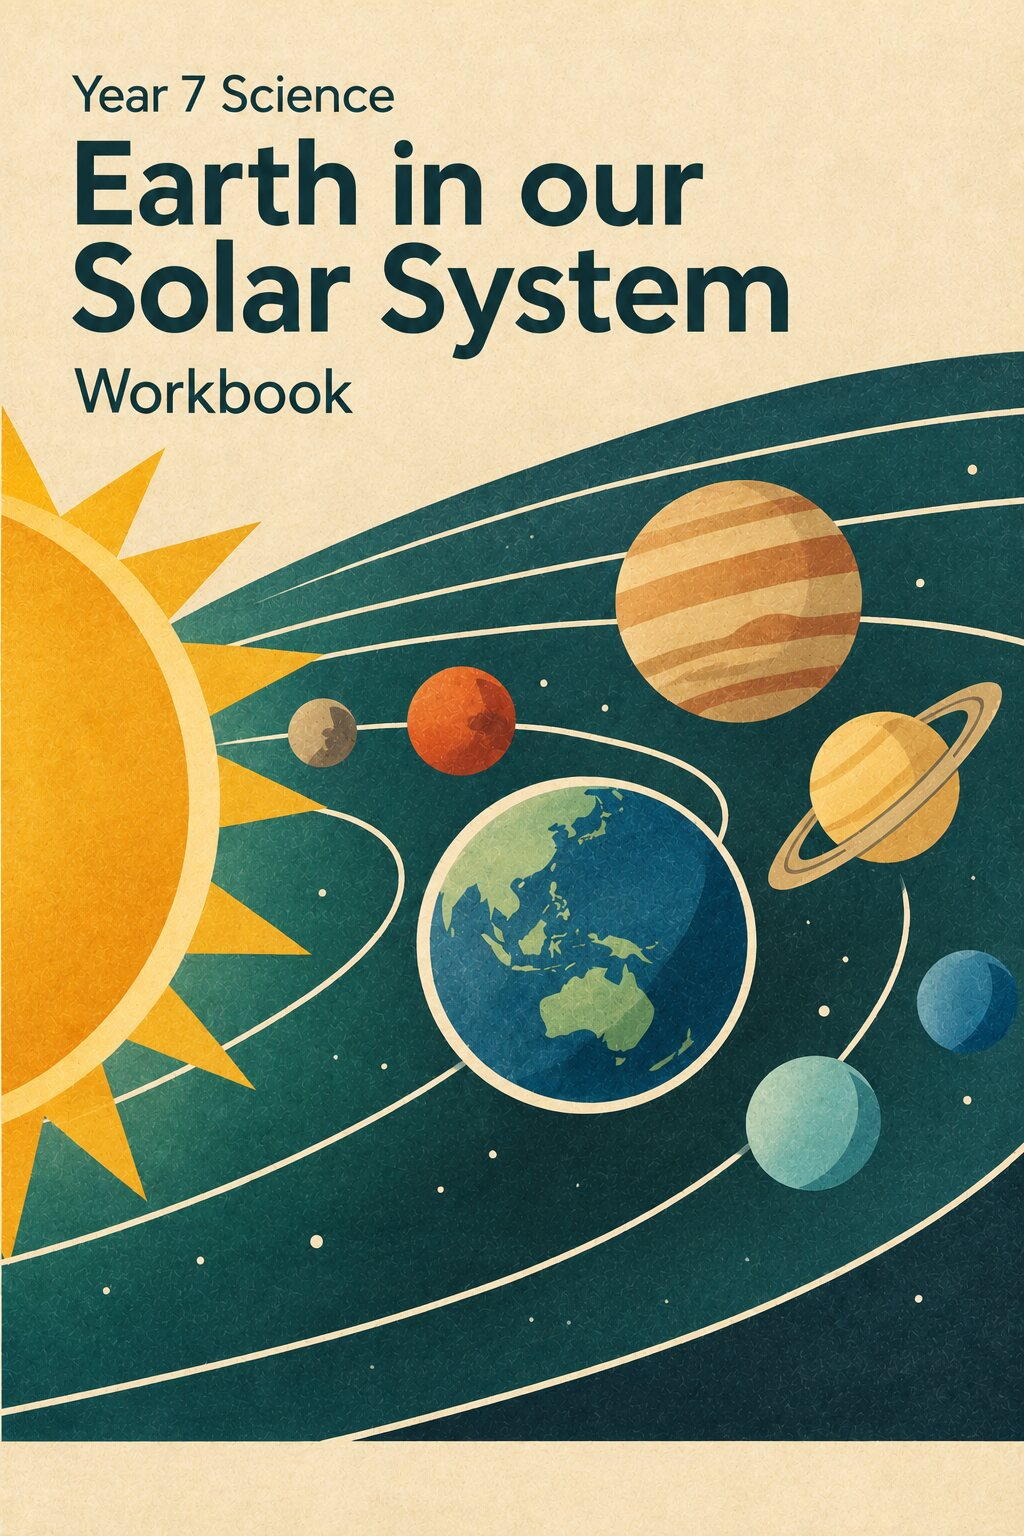
\includegraphics[width=\paperwidth, height=\paperheight, keepaspectratio=false, trim=0 40 0 40, clip]{../../../covers/earth-solar-system.jpg}};
  \node[anchor=north east, fill=white, draw=Ink, line width=0.6pt, rounded corners=1.5mm,
        inner xsep=2.4mm, inner ysep=2mm, text width=33mm, font=\headingfont\footnotesize]
    at ([xshift=-5mm, yshift=-4.5mm]current page.north east)
    {\textbf{Name}\par\vspace{4.2mm}\hrule\vspace{2.2mm}\textbf{Class}\par\vspace{4.2mm}\hrule};
  \node[anchor=south east, fill=white, draw=Ink, line width=0.6pt, rounded corners=1.2mm,
        inner xsep=2.6mm, inner ysep=2mm, font=\headingfont\bfseries, align=right]
    at ([xshift=-5mm, yshift=6mm]current page.south east)
    {Advanced Space\\[-1pt]{\normalfont\headingfont\scriptsize Topics 1--5}};
\end{tikzpicture}
\mbox{}
\clearpage

\thispagestyle{plain}\markboth{Advanced Space}{Advanced Space}
{\headingfont\bfseries\Large Advanced Space}\par
{\headingfont Topics 1--5 \textbullet\ Above the Year 7 level}\par\vspace{5mm}
\renewcommand{\arraystretch}{2.2}
\begin{tabular}{@{}l p{78mm}@{}}
\textbf{Name} & \hrulefill \\ \textbf{Class} & \hrulefill \\ \textbf{Teacher} & \hrulefill \\
\end{tabular}
\renewcommand{\arraystretch}{1}

\begin{countrybox}{Acknowledgement of Country}
This booklet was created on the unceded Country of the Wurundjeri-Woiwurrung people of the Kulin Nation. We acknowledge Elders past, present, and emerging. Aboriginal and Torres Strait Islander peoples have read, recorded and navigated by this sky for tens of thousands of years --- the oldest continuous astronomical tradition on Earth --- and that knowledge appears throughout this unit as living science, not history.
\end{countrybox}

\begin{keybox}{How this booklet works}
\textbf{Advanced Space} goes deeper into the ideas of the lesson book: more powerful models, the mathematics behind them, and harder problems that bring several ideas together. Each topic builds on the lessons named in the contents. Each kind of box has its own frame and mark:\par\smallskip
\renewcommand{\arraystretch}{1.35}
\begin{tabular}{@{}p{24mm}l@{}}
\textbf{I do} {\scriptsize\textbullet} & Worked through for you --- follow it \\
\textbf{We do} {\scriptsize\textbullet\textbullet} & You try it with help \\
\textbf{You do} {\scriptsize\textbullet\textbullet\textbullet} & On your own: check your understanding \\
\textbf{Key idea} & The idea to remember \\
\textbf{Reading} & A deeper reading (double frame) \\
\textbf{Country} & First Nations perspectives (dotted frame) \\
\end{tabular}
\end{keybox}

\clearpage\markboth{Contents}{Contents}
\subsection*{Contents}
\renewcommand{\arraystretch}{1.35}
\begin{tabular}{|>{\Centering}p{11mm}|>{\RaggedRight}p{52mm}|>{\Centering}p{15mm}|>{\Centering}p{13mm}|}
  \hline\thead{Topic} & \thead{Title} & \thead{Deepens lesson} & \thead{Page} \\ \hline
  1 & \hyperlink{lesson.1.1}{The Moon Up Close} & 1, 3, 4 & \hyperlink{lesson.1.1}{p.\ \pageref{sec:1}} \\ \hline
  2 & \hyperlink{lesson.2.1}{Earth's Shield and Crowded Orbits} & 1, 6 & \hyperlink{lesson.2.1}{p.\ \pageref{sec:2}} \\ \hline
  3 & \hyperlink{lesson.3.1}{The Search for Life} & 5, 6 & \hyperlink{lesson.3.1}{p.\ \pageref{sec:3}} \\ \hline
  4 & \hyperlink{lesson.4.1}{Gravity and Orbits} & 1, 3, 5 & \hyperlink{lesson.4.1}{p.\ \pageref{sec:4}} \\ \hline
  5 & \hyperlink{lesson.5.1}{Stars, Galaxies and Starlight} & 5, 7 & \hyperlink{lesson.5.1}{p.\ \pageref{sec:5}} \\ \hline
  --- & \hyperlink{glossary}{Glossary} & & \hyperlink{glossary}{\pageref{sec:glossary}} \\ \hline
\end{tabular}
\renewcommand{\arraystretch}{1}
% ══════════════════════════════════════════════════════════════════════════════
%  ADVANCED SPACE — the above-level book (from 2027)
%  Faculty decision, Nov 2026: every student completes the at-level lesson book;
%  students who excel move on to this book. Its topics go deeper into the ideas
%  of the at-level lessons rather than adding more of the same work.
%
%  Topics 1 and 2 are written here around the master's Year 8 extension boxes
%  from Lessons 1, 3, 4 and 6 (%%ABOVE:n%%, n counting them in the order they
%  appear in Lessons 1-7: 1-2 Lesson 1, 3 Lesson 3, 4 Lesson 4, 5 Lesson 6,
%  6 Lesson 7). Topics 3-5 are the master's Lessons 8-10, whole (%%LESSON:n%%);
%  Lesson 7's extension box closes Topic 5. Built by make_a5.py.
% ══════════════════════════════════════════════════════════════════════════════

% ══════════════════════════════════════════════════════════════════════════════
%  TOPIC 1 — THE MOON UP CLOSE                         (deepens Lessons 1, 3, 4)
% ══════════════════════════════════════════════════════════════════════════════
\setcounter{section}{0}
\lessonopener{1}{The Moon Up Close}{../art/l3-ink.pdf}{1 \textbullet\ The Moon Up Close}\label{sec:1}\pdfbookmark[1]{Topic 1}{lesson.1}\hypertarget{lesson.1.1}{}
\vc{Deepens Lessons 1, 3 and 4}{Where the Moon came from; why eclipses are rare; how the Moon's orbit is growing}

\begin{keyvocab}
  \vocabrow{Giant Impact Hypothesis}
  \vocabrow{Isotope}
  \vocabrow{Node}
  \vocabrow{Saros cycle}
  \vocabrow{Angular size}
  \vocabrow{Annular eclipse}
  \vocabrow{Recession}
\end{keyvocab}

\subsection{Where the Moon came from}\label{sub:a1.1}

Every rock has a chemical fingerprint. Elements come in slightly different versions, called \vocab{isotope}\label{voc:isotope}s, and the mix of oxygen isotopes in a rock depends on where in the early solar system its material formed. That fingerprint is the key evidence in the reading below.

\begin{abovebox}[Reading \textbullet\ How the Moon formed --- the Giant Impact Hypothesis]
The leading model for the Moon's origin is the \vocab{Giant Impact Hypothesis}\label{voc:giant-impact-hypothesis}. About \textbf{4.5 billion years ago} a Mars-sized body --- named \textbf{Theia} --- struck the young Earth. The collision threw a disc of molten rock and vapour into orbit, and that material clumped together under gravity to form the Moon.
	
	\medskip
	Two pieces of evidence support it:
	\begin{itemize}
		\item The Moon has almost \textbf{no iron core}. Earth's iron had already sunk to its centre before the impact, so the debris blasted into orbit came mostly from the rocky mantle.
		\item Moon rock returned by the Apollo missions has \textbf{oxygen isotope ratios identical to Earth's}. Rock formed elsewhere in the solar system does not match --- so the Moon and Earth are made of the same material.
	\end{itemize}
	
	\medskip
	\textbf{Why it matters}: the Moon's mass stabilises Earth's axial tilt at about 23.5°. Without it, the tilt could wander between 0° and 85° over millions of years, making stable long-term climates --- and possibly complex life --- far less likely.
\end{abovebox}


\begin{youdobox}
\question{2}{Describe the Giant Impact Hypothesis in two sentences.}
\answerbox{1.6cm}

\question{2}{Explain how each of the two pieces of evidence supports it.}
\answerbox{1.6cm}

\question{2}{An earlier idea was that the Moon was a passing body captured by Earth's gravity. Which piece of evidence counts most strongly against this? Explain.}
\answerbox{1.6cm}
\end{youdobox}

\subsection{Why eclipses are rare}\label{sub:a1.2}

\begin{abovebox}[Reading \textbullet\ Eclipse geometry]
Eclipses don't happen every New or Full Moon because the Moon's orbit is tilted 5.1° relative to Earth's orbit around the Sun. Eclipses only occur when a New or Full Moon coincides with the Moon being at a \vocab{node}\label{voc:node} (one of two points where its orbit crosses the ecliptic). The pattern of eclipses repeats every 18 years, 11 days, 8 hours --- the \vocab{Saros cycle}\label{voc:saros-cycle}.
	
	\medskip
	\textbf{Why the Moon fits the Sun perfectly}: The Moon is 400$\times$ smaller than the Sun but 400$\times$ closer. Their angular diameters in our sky are almost identical --- making total solar eclipses possible. This is unique in our solar system.
\end{abovebox}


How big something looks in the sky is its \vocab{angular size}\label{voc:angular-size}. It depends on two things: its real size and how far away it is. Two objects look the same size when their diameter divided by their distance is the same.

\begin{idobox}{Do the Sun and Moon really look the same size?}
Sun: diameter 1\,392\,000\,km, distance 150\,000\,000\,km.\quad $1\,392\,000 \div 150\,000\,000 = 0.0093$\\
Moon: diameter 3474\,km, distance 384\,400\,km.\quad $3474 \div 384\,400 = 0.0090$

\smallskip
The two numbers are almost equal, so the Moon only just covers the Sun. When the Moon is a little further away than average, it does not quite cover it, and a ring of Sun shows around it: an \vocab{annular eclipse}\label{voc:annular-eclipse}.
\end{idobox}

\begin{wedobox}{Eclipses in the far future}
The Moon moves away from Earth by about 3.8\,cm a year (its \vocab{recession}\label{voc:recession}). In 600 million years, how much further away will it be, in kilometres? (1\,km $=$ 100\,000\,cm.) Calculate its new diameter-to-distance number, and decide whether total eclipses of the Sun will still happen.
\workbox{5.0cm}
\end{wedobox}

\subsection{A growing orbit}\label{sub:a1.3}

\begin{abovebox}[Reading \textbullet\ How much closer was the Moon?]
Kepler's third law says the square of an orbital period is proportional to the
cube of the orbital radius: $T^2 \propto r^3$, so $r \propto T^{2/3}$.

At 635 Ma there were 13.1 lunar months in a year; today there are 12.37. Since
the year itself has not changed length, the month was
$12.37 / 13.1 = 0.944$ times as long as it is now. Therefore

\[ \frac{r_{635}}{r_{\text{now}}} = 0.944^{2/3} = 0.963 \]

so the Moon sat at about $0.963 \times 384{,}400 \approx 370{,}000$ km ---
roughly \textbf{14,000 km closer}, or 3.7\%. Spread over 635 million years that
is an average recession of about 2.2 cm per year, which is where the figure in
Section 3.1 comes from. Notice what this does \emph{not} say: the Moon was not
dramatically closer in the Precambrian. The interesting result is the
\textbf{rate}, not the distance.

\medskip
\noindent\textbf{Try it:} the Moon's distance is measured today as 384,400 km
and it recedes at 3.8 cm per year. If that rate had always applied, how far
away was the Moon 635 million years ago? Compare your answer with the 14,000 km
above, and say what the difference tells you.
\workbox{3.5cm}
\end{abovebox}


\begin{youdobox}[Challenge]
\question{4}{Use what you have learnt in this topic to explain why the people living in 600 million years will never see a total eclipse of the Sun, and why the people living 600 million years ago saw them more often than we do. Include numbers.}
\workbox{5.0cm}
\end{youdobox}

% ══════════════════════════════════════════════════════════════════════════════
%  TOPIC 2 — EARTH'S SHIELD AND CROWDED ORBITS             (deepens Lessons 1, 6)
% ══════════════════════════════════════════════════════════════════════════════
\setcounter{section}{1}
\lessonopener{2}{Earth's Shield and Crowded Orbits}{../art/l6-ink.pdf}{2 \textbullet\ Earth's Shield and Crowded Orbits}\label{sec:2}\pdfbookmark[1]{Topic 2}{lesson.2}\hypertarget{lesson.2.1}{}
\vc{Deepens Lessons 1 and 6}{Earth's magnetic field and space weather; the energy of orbital debris; who looks after near-Earth space}

\begin{keyvocab}
  \vocabrow{Dynamo effect}
  \vocabrow{Magnetosphere}
  \vocabrow{Solar wind}
  \vocabrow{Space weather}
  \vocabrow{Kinetic energy}
  \vocabrow{Kessler syndrome}
  \vocabrow{Tragedy of the commons}
\end{keyvocab}

\subsection{Earth's magnetic shield}\label{sub:a2.1}

\begin{abovebox}[Reading \textbullet\ Earth's magnetosphere and space weather]
The liquid iron in Earth's \textbf{outer core} is constantly moving, and moving
	metal generates a magnetic field --- the \vocab{dynamo effect}\label{voc:dynamo-effect}. That field does
	not stop at the surface. It reaches tens of thousands of kilometres out into
	space, forming the \vocab{magnetosphere}\label{voc:magnetosphere}: an invisible shield around the whole
	planet.
	
	\smallskip
	It has something to shield us from.
	
	\begin{itemize}
		\item \vocab{Solar wind}\label{voc:solar-wind} --- a constant stream of charged particles blowing
		outward from the Sun at 400--800 km/s. It never stops.
		\item \vocab{Coronal mass ejections}\label{voc:coronal-mass-ejections} (CMEs) --- huge bursts of plasma thrown
		off the Sun, which can reach Earth in one to three days.
		\item \vocab{Auroras}\label{voc:auroras} --- the magnetosphere funnels charged particles toward
		the poles, where they collide with atmospheric gases and make them glow.
		This is the \textit{aurora australis} in the south and the
		\textit{aurora borealis} in the north. An aurora is what the shield
		looks like while it is working.
	\end{itemize}
	
	\smallskip
	\vocab{Space weather}\label{voc:space-weather} is the name for these events, and it has consequences on
	the ground. On 13 March 1989 a geomagnetic storm induced currents in Quebec's
	power transmission lines large enough to collapse the entire provincial grid in
	under 90 seconds, leaving about six million people without electricity for nine
	hours. Modern GPS, satellites and radio communication are all vulnerable.
	
	\medskip
	\noindent\textbf{Challenge.}\; Mars has no global magnetic field, and
	most of its atmosphere has been stripped away by the solar wind over billions of
	years. Earth has both a field and an atmosphere. What does the comparison suggest
	the magnetic field is doing --- and what might happen if Earth's field weakened
	a great deal?
	\workbox{5.0cm}
\end{abovebox}


\begin{youdobox}
\question{2}{Explain where Earth's magnetic field comes from.}
\answerbox{1.6cm}

\question{2}{Why are auroras seen mostly near the poles?}
\answerbox{1.6cm}

\question{2}{Name two kinds of technology that space weather can damage, and why.}
\answerbox{1.6cm}
\end{youdobox}

\subsection{Why a fleck of paint is dangerous}\label{sub:a2.2}

Satellites in low orbit travel at about 7.5\,km every second. At that speed, even tiny pieces of debris carry enormous \vocab{kinetic energy}\label{voc:kinetic-energy}, the energy of movement. A fleck of paint once chipped a window of a Space Shuttle. In 1978 the NASA scientist Donald Kessler warned that if enough debris builds up, one collision would make fragments that cause more collisions, which make more fragments, until some orbits became unusable. This runaway chain is called the \vocab{Kessler syndrome}\label{voc:kessler-syndrome}.

\begin{idobox}{The energy of a fragment}
\[ \text{kinetic energy (J)} = \tfrac{1}{2} \times \text{mass (kg)} \times \text{speed (m/s)}^2 \]
A 1.4\,g fragment of aluminium (0.0014\,kg) at 7500\,m/s:\\
$\tfrac{1}{2} \times 0.0014 \times 7500^2 = 0.0007 \times 56\,250\,000 \approx \mathbf{39\,000\ J}$\\
That is about the kinetic energy of a one-tonne car at 32\,km/h, all delivered to a spot smaller than a fingernail.
\end{idobox}

\begin{wedobox}{A lost bolt}
A 10\,g bolt (0.010\,kg) drifts away from a spacewalk at orbital speed, 7500\,m/s. Calculate its kinetic energy. How many times more is that than the aluminium fragment?
\workbox{4.5cm}
\end{wedobox}

Removing debris is expensive, and whoever pays for it helps every other satellite owner as much as themselves. Economists call this the \vocab{tragedy of the commons}\label{voc:tragedy-of-the-commons}: when something is shared by everyone, no single owner has a reason to pay to look after it, so it is overused and damaged.

\begin{abovebox}[Reading \textbullet\ Active debris removal and orbital governance]
Active debris removal (ADR) technologies in development include robotic arm capture (ESA ClearSpace-1), electromagnetic tether deorbit (JAXA ELSA-d), and laser ablation. The fundamental challenge is economic: removing debris benefits all space users, not just the company paying for removal --- a classic ``tragedy of the commons.'' Proposed governance solutions include binding UN agreements, debris levies on satellite operators, and mandatory deorbit insurance. Current international frameworks (Outer Space Treaty 1967, UN COPUOS guidelines) are non-binding and insufficient for the scale of the problem.
\end{abovebox}


\begin{youdobox}[Challenge]
\question{4}{Explain why the Kessler syndrome could make a crowded orbit unusable even if no one launched anything new. Then propose one rule that every country launching satellites should follow, and explain why it would be hard to get every country to agree.}
\workbox{5.0cm}
\end{youdobox}

% ══════════════════════════════════════════════════════════════════════════════
%  TOPICS 3-5 — THE MASTER'S LESSONS 8-10, WHOLE
% ══════════════════════════════════════════════════════════════════════════════
\setcounter{section}{2}
\lessonopener{3}{The Search for Life --- Astrobiology}{../art/l8-ink.pdf}{3 \textbullet\ The Search for Life}\label{sec:3}\pdfbookmark[1]{Topic 3}{lesson.3}\hypertarget{lesson.3.1}{}
\vc{Science Understanding}{Biological sciences: Conditions for life; Earth and space sciences: Habitable zones; exoplanets}

\begin{keyvocab}
  \vocabrow{Liquid water}
  \vocabrow{Carbon chemistry}
  \vocabrow{Energy source}
  \vocabrow{Stable environment}
  \vocabrow{Habitable zone}
  \vocabrow{Tidal heating}
  \vocabrow{Mars}
  \vocabrow{Europa}
  \vocabrow{Enceladus}
  \vocabrow{Extremophiles}
  \vocabrow{Transit method}
  \vocabrow{Radial velocity}
  \vocabrow{Biosignatures}
\end{keyvocab}

\subsection{Requirements for life as we know it}\label{sub:8.1}

\begin{wedobox}{Entry task: what does life actually need?}
Sort the eight conditions into the two columns, then rank the four you think
matter most. Do this \textbf{before} you read on --- you are predicting, not
looking it up.

\medskip
\noindent\textbf{Sort these:}\; liquid water \;\textbullet\; oxygen atmosphere
\;\textbullet\; carbon chemistry \;\textbullet\; sunlight \;\textbullet\; an
energy source \;\textbullet\; a magnetic field \;\textbullet\; a stable
environment over time \;\textbullet\; moderate temperature

\medskip
\begin{center}
\begin{fillin}[2.9]
\begin{tfitbox}\begin{tabular}{|p{5.48cm}|p{5.48cm}|}
\hline
\textbf{Required for life as we know it} & \textbf{Not required (but might help)} \\ \hline
 & \\ \hline
 & \\ \hline
 & \\ \hline
 & \\ \hline
\end{tabular}\end{tfitbox}
\end{fillin}
\end{center}

\noindent\textbf{My top four, most important first --- and why:}
\answerbox{5.0cm}
\end{wedobox}


Life on Earth requires:
\begin{itemize}
  \item \vocab{Liquid water}\label{voc:liquid-water}: as a solvent for biochemical reactions
  \item \vocab{Carbon chemistry}\label{voc:carbon-chemistry}: carbon forms 4 bonds and chains of any length --- uniquely suited to the complexity life requires (CHNOPS elements: Carbon, Hydrogen, Nitrogen, Oxygen, Phosphorus, Sulfur)
  \item \vocab{Energy source}\label{voc:energy-source}: sunlight (photosynthesis) or chemical energy (chemosynthesis)
  \item \vocab{Stable environment}\label{voc:stable-environment}: over geological timescales for evolution
\end{itemize}


\begin{youdobox}

\question{2}{List the four requirements for life as we know it.}
\answerbox{1.6cm}

\question{2}{Explain why carbon is uniquely suited to the chemistry of life.}
\answerbox{1.6cm}

\end{youdobox}

\subsection{The habitable zone}\label{sub:8.2}

The \vocab{habitable zone}\label{voc:habitable-zone} (``Goldilocks zone'') is the range of distances from a star where liquid water can exist on a planet's surface. Earth is well within the Sun's habitable zone. Mars is on the outer edge.

\begin{keybox}{Beyond the habitable zone: tidal heating}
\vocab{Tidal heating}\label{voc:tidal-heating} --- gravitational flexing by a parent planet --- can maintain liquid water far outside the classical habitable zone. This is why Europa (Jupiter's moon) and Enceladus (Saturn's moon) are high-priority astrobiology targets despite being far from the Sun.
\end{keybox}


\begin{youdobox}

\question{2}{Define the habitable zone and state where Earth and Mars sit relative to it.}
\answerbox{1.6cm}

\question{3}{Explain how tidal heating allows liquid water to exist far outside the classical habitable zone.}
\answerbox{1.6cm}

\end{youdobox}

\subsection{Promising targets in our solar system}\label{sub:8.3}

\begin{itemize}
  \item \vocab{Mars}\label{voc:mars}: ancient river channels, delta deposits, and lake beds confirm liquid water billions of years ago. Possible present-day liquid brines under the southern polar ice cap. Perseverance rover collecting samples for return to Earth
  \item \vocab{Europa}\label{voc:europa}: 10--30 km ice shell over a global saltwater ocean; tidal heating from Jupiter; probable hydrothermal vents on ocean floor. Europa Clipper (NASA, 2024) will flyby 49 times
  \item \vocab{Enceladus}\label{voc:enceladus}: active water geysers from cracks in its icy shell; Cassini detected H$_2$, CO$_2$, and organic molecules in the plume --- a potential chemical energy source for life
\end{itemize}


\begin{youdobox}

\question{2}{State two pieces of evidence that Mars once had liquid water.}
\answerbox{1.6cm}

\question{3}{Describe the structure of Europa that makes it a high-priority astrobiology target.}
\answerbox{1.6cm}

\question{3}{State what Cassini detected in the plume of Enceladus, and explain why this matters for the search for life.}
\answerbox{1.6cm}

\end{youdobox}

\subsection{Extremophiles}\label{sub:8.4}

\vocab{Extremophiles}\label{voc:extremophiles} are organisms that thrive in conditions once thought impossible for life:
\begin{itemize}
  \item Hydrothermal vents (no sunlight, extreme pressure, 400°C water)
  \item Antarctic ice (-20°C)
  \item Highly acidic environments (pH 0)
  \item Highly radioactive environments (Deinococcus radiodurans)
\end{itemize}
Their existence vastly expands the range of environments where we search for life elsewhere.


\begin{youdobox}

\question{3}{Define ``extremophile'' and give two examples of the extreme conditions they tolerate.}
\answerbox{1.6cm}

\question{2}{Explain how the discovery of extremophiles changed where scientists search for life beyond Earth.}
\answerbox{1.6cm}

\end{youdobox}

\subsection{Exoplanets and biosignatures}\label{sub:8.5}

More than 5,500 exoplanets confirmed (2024). Detection methods:
\begin{itemize}
  \item \vocab{Transit method}\label{voc:transit-method}: planet passes in front of star; brightness dips slightly; detects size and orbital period
  \item \vocab{Radial velocity}\label{voc:radial-velocity}: planet makes star wobble; detected as Doppler shifts; detects mass
\end{itemize}

\vocab{Biosignatures}\label{voc:biosignatures}: chemical signs of life detectable at a distance. Oxygen + methane together are a strong biosignature (both are destroyed by each other unless continuously replenished by living processes). JWST has already detected CO$_2$ on exoplanet WASP-39b; detecting O$_2$ and CH$_4$ together on an Earth-like planet is the next frontier.

\begin{countrybox}{Sky beings and the question of origins}
In Wurundjeri tradition, the creator being Bunjil the Wedge-tailed Eagle flew into the sky after establishing Country and became the star Altair. His sons, the Bram-bram-bult, continue to observe from the sky. Aboriginal Australian cosmologies have always understood the sky as inhabited and relational --- a different, valid framework for the question of what exists beyond our world. Western astrobiology asks whether microbial life exists in Europa's ocean. Aboriginal cosmology asks a different kind of question: about origin, relationship, and meaning. Both are genuine human responses to the same remarkable sky.
\end{countrybox}

\begin{idobox}{Worked example: Drake equation}
\textit{Using the Drake equation with optimistic values: $R_* = 3$/yr, $f_p = 1$, $n_e = 0.1$, $f_l = 1$, $f_i = 0.1$, $f_c = 0.1$, $L = 10{,}000$ years. Estimate N (civilisations in the Milky Way).}

$N = 3 \times 1 \times 0.1 \times 1 \times 0.1 \times 0.1 \times 10{,}000 = \mathbf{30}$

With pessimistic estimates (especially short $L$), N could be less than 1. The equation is a framework for identifying what we don't know rather than a precise answer.
\end{idobox}

\begin{wedobox}{Your turn --- Life on Europa}
Construct a scientific argument for whether life might exist in Europa's subsurface ocean. Include: (a) conditions present; (b) an Earth analogue; (c) missing evidence; (d) how you would obtain it.

\vspace{6cm}
\end{wedobox}


\begin{youdobox}

\question{1}{State approximately how many exoplanets had been confirmed by 2024.}
\answerbox{1.6cm}

\question{3}{Explain the transit method of exoplanet detection and state what it reveals about the planet.}
\answerbox{1.6cm}

\question{3}{Explain why oxygen and methane detected together are considered a strong biosignature.}
\answerbox{1.6cm}

\end{youdobox}

\clearpage
\begin{abovebox}[Reading \textbullet\ The Fermi Paradox]

Given the size and age of the universe, intelligent life should be detectable --- yet we detect nothing. Proposed resolutions include: (1) Rare Earth hypothesis (complex life is extraordinarily rare); (2) Great Filter (a catastrophic barrier that most civilisations don't survive); (3) communication limits (light-speed travel; we've only been broadcasting for $\sim$100 years in a galaxy 100,000 light-years across); (4) non-radio technologies we don't recognise. The Breakthrough Listen initiative uses Parkes and other telescopes in systematic SETI searches. No confirmed signal has ever been received.
\end{abovebox}
\setcounter{section}{3}
\lessonopener{4}{Gravity and Orbits}{../art/l9-ink.pdf}{4 \textbullet\ Gravity and Orbits}\label{sec:4}\pdfbookmark[1]{Topic 4}{lesson.4}\hypertarget{lesson.4.1}{}
\vc{Science Understanding}{Physical sciences: Gravitational force; orbital motion; Newton's law of universal gravitation}

\begin{keyvocab}
  \vocabrow{Orbit}
  \vocabrow{Free fall}
\end{keyvocab}

\subsection{Newton's law of universal gravitation}\label{sub:9.1}

Every object with mass attracts every other object with mass:

\begin{center}
\Large $F = \dfrac{G \cdot m_1 \cdot m_2}{r^2}$
\end{center}

Where: $F$ = gravitational force (N), $G$ = gravitational constant ($6.67 \times 10^{-11}$ N\,m$^2$/kg$^2$), $m_1, m_2$ = masses (kg), $r$ = distance between centres (m).

\begin{itemize}
  \item Double either mass $\rightarrow$ force doubles
  \item Double the distance $\rightarrow$ force decreases to \textbf{one quarter} (inverse square law)
  \item Gravity is always \textit{attractive} --- it only pulls, never pushes
\end{itemize}


\begin{youdobox}

\question{3}{Write Newton's law of universal gravitation and state what each symbol represents.}
\answerbox{1.6cm}

\question{1}{State what happens to the gravitational force between two objects if one of the masses is quadrupled.}
\answerbox{1.6cm}

\question{2}{Explain what happens to the gravitational force if the distance between two objects is doubled, and name this relationship.}
\answerbox{1.6cm}

\question{1}{A student claims gravity can push objects apart. Explain why this is incorrect.}
\answerbox{1.6cm}

\end{youdobox}

\subsection{Orbital motion}\label{sub:9.2}

\begin{wedobox}{Entry task: Newton's cannonball}
A cannon sits on top of an impossibly tall mountain and fires horizontally.
On the diagram, sketch the path of the cannonball when it is fired
\textbf{(a)} slowly, \textbf{(b)} faster, and \textbf{(c)} fast enough that it
never lands. Label each path.

\begin{center}
\begin{fitbox}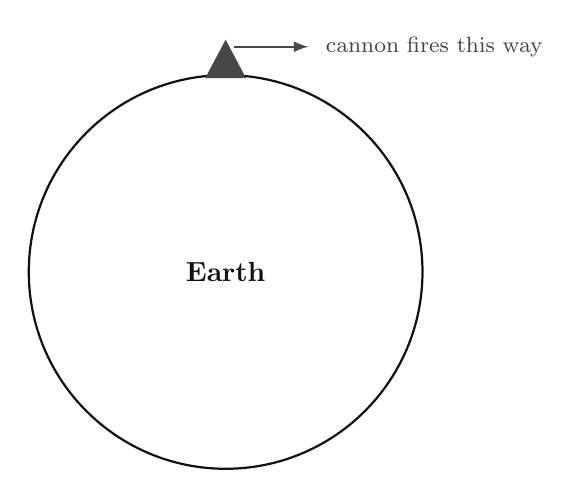
\begin{tikzpicture}
  \fill[SpaceLight] (0,0) circle (2.5cm);
  \draw[Space, thick] (0,0) circle (2.5cm);
  \node[Space, font=\headingfont\bfseries] at (0,0) {Earth};
  \fill[DarkGrey] (-0.26,2.46) -- (0,2.95) -- (0.26,2.46) -- cycle;
  \draw[DarkGrey, thick, -latex] (0.10,2.86) -- (1.05,2.86);
  \node[DarkGrey, font=\footnotesize, anchor=west] at (1.15,2.86) {cannon fires this way};
\end{tikzpicture}\end{fitbox}
\end{center}

\noindent\textbf{Is the cannonball in path (c) still falling? Explain.}
\answerbox{5.0cm}
\end{wedobox}


An \vocab{orbit}\label{voc:orbit} occurs when gravity provides the centripetal force needed to keep an object moving in a curved path. Orbiting objects are in constant \vocab{free fall}\label{voc:free-fall} toward the body they orbit --- but moving forward so fast they keep missing it.


Higher altitude = lower orbital speed (and longer period):

\begin{center}
	\begin{tfitbox}\begin{tabular}{llrr}
		\toprule
		\textbf{Orbit} & \textbf{Altitude} & \textbf{Speed} & \textbf{Period} \\
		\midrule
		LEO (ISS) & 200--2,000 km & $\approx$7.9 km/s & $\approx$90 min \\
		MEO (GPS) & 2,000--35,786 km & $\approx$3.9 km/s & $\approx$12 h \\
		GEO (comms, weather) & 35,786 km & $\approx$3.1 km/s & 24 h \\
		\bottomrule
	\end{tabular}\end{tfitbox}
\end{center}

\begin{keybox}{Why astronauts appear weightless}
The ISS orbits at $\approx$408 km altitude, where gravity is about 90\% of surface strength. Astronauts appear weightless because they \textit{and} the station are falling together at the same rate. ``Weightlessness'' is free fall --- not absence of gravity.
\end{keybox}


\begin{youdobox}

\question{2}{Define an orbit, referring to gravity and centripetal force.}
\answerbox{1.6cm}

\question{3}{Explain why an object in orbit is described as being in constant free fall.}
\answerbox{1.6cm}

\question{2}{State the approximate altitude of the ISS and the strength of gravity there as a percentage of its strength at Earth's surface.}
\answerbox{1.6cm}

\question{2}{A student says astronauts float on the ISS because there is no gravity in space. Correct this statement.}
\answerbox{1.6cm}

\end{youdobox}


\begin{idobox}{Worked example: Weight at ISS altitude}
\textit{An astronaut weighs 700 N on Earth (radius 6,371 km). What is their weight at ISS altitude (408 km above surface)?}

$r_\text{ISS} = 6{,}371 + 408 = 6{,}779$ km

Force ratio $= \left(\dfrac{6{,}371}{6{,}779}\right)^2 = 0.883$

Weight at ISS $= 700 \times 0.883 = \mathbf{618 \text{ N}}$ (about 88\% of surface weight)
\end{idobox}

\clearpage
\begin{abovebox}[Reading \textbullet\ Escape velocity]

To escape a planet's gravitational field entirely: $v_e = \sqrt{\dfrac{2GM}{r}}$

Earth: 11.2 km/s \quad Moon: 2.4 km/s \quad Mars: 5.0 km/s \quad Jupiter: 59.5 km/s

The Moon's low escape velocity explains why it has no atmosphere: gas molecules moving at thermal speeds can escape to space over time.
\end{abovebox}



\begin{youdobox}

\question{2}{Using the table, state the orbital speed and period of the ISS.}
\answerbox{1.6cm}

\question{2}{Describe the relationship between orbital altitude and orbital speed shown in the table.}
\answerbox{1.6cm}

\question{2}{Explain why a satellite in geostationary orbit appears to stay in the same place in the sky.}
\answerbox{1.6cm}

\question{2}{GPS satellites operate in MEO. Using the table, state the altitude range and orbital period of this orbit.}
\answerbox{1.6cm}

\end{youdobox}
\setcounter{section}{4}
\lessonopener{5}{Stars, Galaxies and Starlight}{../art/l10-ink.pdf}{5 \textbullet\ Stars, Galaxies and Starlight}\label{sec:5}\pdfbookmark[1]{Topic 5}{lesson.5}\hypertarget{lesson.5.1}{}
\vc{Science Understanding}{Earth and space sciences: Properties of stars; galaxies; scale of the universe}

\begin{keyvocab}
  \vocabrow{Light-year}
  \vocabrow{Main sequence}
  \vocabrow{Giant branch}
  \vocabrow{White dwarfs}
  \vocabrow{Electromagnetic spectrum}
  \vocabrow{Refracting telescopes}
  \vocabrow{Reflecting telescopes}
  \vocabrow{Radio telescopes}
  \vocabrow{Space telescopes}
  \vocabrow{Absorption lines}
  \vocabrow{Composition}
  \vocabrow{Temperature}
  \vocabrow{Velocity}
  \vocabrow{Virtual telescope}
  \vocabrow{Interferometry}
\end{keyvocab}

\needspace{5\baselineskip}
\vspace{0.8em}
{\headingfont\large\bfseries\color{Navy}Part A --- Stars and Galaxies}
\vspace{0.2em}

\noindent{\color{Gold}\rule{\linewidth}{1.2pt}}
\vspace{0.6em}



\subsection{Light-years and stellar distances}\label{sub:10.1}

\begin{wedobox}{Entry task: which unit fits which distance?}
Complete the table. For each distance, choose the unit that gives a sensible
number --- kilometres, astronomical units (AU) or light-years --- and fill in
the blanks.

\medskip
\begin{center}
\begin{fillin}
\begin{tfitbox}\begin{tabular}{|p{4.25cm}|p{2.83cm}|p{3.46cm}|}
\hline
\textbf{Distance} & \textbf{Best unit} & \textbf{Approximate value} \\ \hline
Earth to the Moon & & 384,400 km \\ \hline
Earth to the Sun & AU & \\ \hline
To the nearest star (Proxima Centauri) & & 4.2 light-years \\ \hline
Diameter of the Milky Way & light-years & \\ \hline
\end{tabular}\end{tfitbox}
\end{fillin}
\end{center}

\noindent\textbf{Why would it be silly to give the Milky Way's diameter in
kilometres?}
\answerbox{5.0cm}
\end{wedobox}


A \vocab{light-year}\label{voc:light-year} is the distance light travels in one year: approximately $9.46 \times 10^{12}$ km (9.46 trillion km). It is a unit of \textit{distance}, not time.

\begin{itemize}
  \item The Sun: light takes 8 min 20 s to reach Earth
  \item Proxima Centauri (nearest star): 4.2 light-years
  \item Milky Way diameter: $\approx$100,000 light-years
  \item Andromeda Galaxy: 2.5 million light-years
\end{itemize}

\begin{keybox}{Looking back in time}
When we observe a star 100 light-years away, we see it as it was 100 years ago --- the light we detect left it then. Telescopes are time machines. JWST images galaxies as they appeared just 300--400 million years after the Big Bang.
\end{keybox}


\begin{youdobox}

\question{2}{Define a light-year and state what type of quantity it measures.}
\answerbox{1.6cm}

\question{2}{Proxima Centauri is 4.2 light-years away. Explain what we are actually seeing when we look at it tonight.}
\answerbox{1.6cm}

\end{youdobox}

\subsection{Star types and the OBAFGKM sequence}\label{sub:10.2}

Stars are classified by surface temperature and colour:

\begin{center}
\begin{tfitbox}\begin{tabular}{lllr}
\toprule
\textbf{Class} & \textbf{Colour} & \textbf{Temperature} & \textbf{Example} \\
\midrule
O & Blue-violet & $>$30,000 K & Zeta Puppis \\
B & Blue-white  & 10,000--30,000 K & Rigel \\
A & White       & 7,500--10,000 K & Sirius \\
F & Yellow-white& 6,000--7,500 K & Procyon \\
G & Yellow      & 5,200--6,000 K & \textbf{The Sun} \\
K & Orange      & 3,700--5,200 K & Arcturus \\
M & Red         & $<$3,700 K & Proxima Centauri \\
\bottomrule
\end{tabular}\end{tfitbox}
\end{center}


\begin{youdobox}

\question{2}{Using the table, state the spectral class and colour of the Sun.}
\answerbox{1.6cm}

\question{3}{Arrange Rigel, the Sun and Proxima Centauri in order of decreasing surface temperature, justifying your order with data from the table.}
\answerbox{1.6cm}

\end{youdobox}

\subsection{Stellar life cycle (sun-like star)}\label{sub:10.3}

\begin{center}
\begin{fitbox}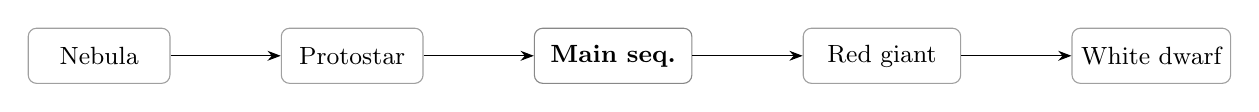
\begin{tikzpicture}[node distance=1.4cm, >=Stealth]
  \node[draw=Space!40, rounded corners=3pt, fill=SpaceLight, font=\small, minimum width=1.8cm, minimum height=0.7cm] (neb) {Nebula};
  \node[draw=Space!40, rounded corners=3pt, fill=SpaceLight, font=\small, minimum width=1.8cm, minimum height=0.7cm, right=of neb] (pro) {Protostar};
  \node[draw=Gold!50, rounded corners=3pt, fill=GoldLight, font=\small, minimum width=2cm, minimum height=0.7cm, right=of pro] (ms) {\textbf{Main seq.}};
  \node[draw=Coral!40, rounded corners=3pt, fill=CoralLight, font=\small, minimum width=2cm, minimum height=0.7cm, right=of ms] (rg) {Red giant};
  \node[draw=Space!40, rounded corners=3pt, fill=SpaceLight, font=\small, minimum width=2cm, minimum height=0.7cm, right=of rg] (wd) {White dwarf};
  \draw[->] (neb) -- (pro);
  \draw[->] (pro) -- (ms);
  \draw[->] (ms) -- (rg);
  \draw[->] (rg) -- (wd);
\end{tikzpicture}\end{fitbox}

\vspace{0.4em}
\small\textit{Massive stars ($>$8 M$_\odot$): Main sequence $\rightarrow$ Red supergiant $\rightarrow$ Supernova $\rightarrow$ Neutron star / Black hole}
\end{center}

\begin{countrybox}{Boorong knowledge: The Magellanic Clouds}
The Large and Small Magellanic Clouds --- dwarf galaxies visible to the naked eye from the Southern Hemisphere --- are incorporated into Boorong star lore as \textit{Yugarilya}, the two Bram-bram-bult (sons of Bunjil the creator), who appear as wedge-tailed eagles in the sky. Aboriginal Australians observed these objects for tens of thousands of years before European astronomers named them after Magellan's 1521 voyage.
\end{countrybox}


\begin{youdobox}

\question{2}{List, in order, the stages in the life cycle of a Sun-like star.}
\answerbox{1.6cm}

\question{2}{State how the life cycle of a star more massive than 8 solar masses differs after the main sequence.}
\answerbox{1.6cm}

\end{youdobox}

\clearpage
\begin{abovebox}[Reading \textbullet\ The Hertzsprung--Russell Diagram]

The H--R diagram plots stellar luminosity (vertical axis) against surface temperature (horizontal axis, running \textit{right to left} --- hot on left). Stars cluster in recognisable zones: the \vocab{main sequence}\label{voc:main-sequence} (a diagonal band), the \vocab{giant branch}\label{voc:giant-branch} (upper right, cool but luminous), and \vocab{white dwarfs}\label{voc:white-dwarfs} (lower left, hot but dim). A star's position reveals its evolutionary stage, mass, and age.
\end{abovebox}

\needspace{5\baselineskip}
\vspace{0.8em}

{\headingfont\large\bfseries\color{Navy}Part B --- Light from Space --- Telescopes and the EM Spectrum}
\vspace{0.2em}

\noindent{\color{Gold}\rule{\linewidth}{1.2pt}}
\vspace{0.6em}

\vc{Science Understanding}{Physical sciences: Electromagnetic radiation; wave properties; telescopes as scientific instruments}

\subsection{The electromagnetic spectrum}\label{sub:10.4}

\begin{wedobox}{Entry task: order the electromagnetic spectrum}
Write the seven regions into the strip in order, longest wavelength on the
left. Then circle the one we can see with our eyes.

\medskip
\noindent\textbf{Word bank:}\; gamma \;\textbullet\; infrared \;\textbullet\;
microwave \;\textbullet\; radio \;\textbullet\; ultraviolet \;\textbullet\;
visible \;\textbullet\; X-ray

\medskip
\begin{center}
\begin{fillin}[3.2]
\begin{tfitbox}\begin{tabular}{|c|c|c|c|c|c|c|}
\hline
\makebox[1.55cm]{} & \makebox[1.55cm]{} & \makebox[1.55cm]{} & \makebox[1.55cm]{} & \makebox[1.55cm]{} & \makebox[1.55cm]{} & \makebox[1.55cm]{} \\ \hline
\end{tabular}\end{tfitbox}
\end{fillin}

\smallskip
{\footnotesize\color{DarkGrey}$\longleftarrow$ longer wavelength, lower energy
\hfill higher energy, shorter wavelength $\longrightarrow$}
\end{center}
\end{wedobox}


Visible light is only a small part of the \vocab{electromagnetic spectrum}\label{voc:electromagnetic-spectrum} (EM spectrum). All EM waves travel at the speed of light ($3 \times 10^8$ m/s) but differ in wavelength and frequency.

\begin{center}
\begin{tfitbox}\begin{tabular}{@{}L{1.83cm}L{1.83cm}L{1.25cm}L{5.20cm}@{}}
\toprule
\textbf{Region} & \textbf{Wavelength} & \textbf{Energy} & \textbf{Astronomical use} \\
\midrule
Radio waves  & mm to km   & Lowest  & Pulsars, CMB, galaxy mapping (Parkes, SKA) \\
Microwaves   & mm         & Low     & CMB, molecular clouds \\
Infrared     & 1\,$\mu$m--1\,mm & Medium-low & Star formation, cool objects, exoplanet atmospheres (JWST) \\
Visible      & 400--700 nm & Medium & Stars, planets, galaxies (optical telescopes) \\
UV           & 10--400 nm  & Medium-high & Hot stars, quasars \\
X-ray        & 0.01--10 nm & High   & Black holes, neutron stars, galaxy clusters \\
Gamma ray    & $<$0.01 nm & Highest & Supernovae, gamma-ray bursts \\
\bottomrule
\end{tabular}\end{tfitbox}
\end{center}


\begin{youdobox}

\question{2}{State one property all electromagnetic waves share, and two properties that differ between them.}
\answerbox{1.6cm}

\question{2}{Using the table, name the region of the spectrum used to study black holes, and the region used to map galaxies with the SKA.}
\answerbox{1.6cm}

\end{youdobox}

\subsection{Telescopes}\label{sub:10.5}

\begin{itemize}
  \item \vocab{Refracting telescopes}\label{voc:refracting-telescopes}: glass lenses bend light to a focus. Limited to small instruments
  \item \vocab{Reflecting telescopes}\label{voc:reflecting-telescopes}: mirrors reflect light to a focus. All major modern telescopes; can be built much larger (Hubble: 2.4 m mirror; JWST: 6.5 m)
  \item \vocab{Radio telescopes}\label{voc:radio-telescopes}: large dish antennas; collect radio waves; Parkes dish (64 m) relayed Moon landing footage
  \item \vocab{Space telescopes}\label{voc:space-telescopes}: above the atmosphere; avoid absorption and blurring; JWST orbits at the Sun--Earth L2 point
\end{itemize}


\begin{youdobox}

\question{2}{Explain the difference between a refracting and a reflecting telescope.}
\answerbox{1.6cm}

\question{2}{Give two reasons for placing a telescope in space rather than on the ground.}
\answerbox{1.6cm}

\end{youdobox}

\subsection{Spectroscopy --- reading starlight}\label{sub:10.6}

When starlight passes through a prism or diffraction grating, \vocab{absorption lines}\label{voc:absorption-lines} appear --- dark lines at specific wavelengths absorbed by elements in the star's outer atmosphere. Each element has a unique spectral fingerprint. From absorption spectra, astronomers determine:
\begin{itemize}
  \item Elemental \vocab{composition}\label{voc:composition} of stars and exoplanet atmospheres
  \item \vocab{Temperature}\label{voc:temperature} (line types reveal temperature class)
  \item \vocab{Velocity}\label{voc:velocity}: blueshifted = moving toward us; redshifted = moving away (Doppler effect)
\end{itemize}

\begin{countrybox}{Wajarri knowledge and the MWA}
The Murchison Widefield Array (MWA) --- precursor to the SKA --- sits on Wajarri Yamatji Country in Western Australia. It maps hydrogen across the Milky Way using radio waves invisible to the naked eye. The Wajarri have observed and named features of this same sky for tens of thousands of years using different instruments (their senses, memory, and song). Both the MWA and Wajarri sky knowledge reveal the same cosmos at different scales and with different tools.
\end{countrybox}

\begin{abovebox}[Reading \textbullet\ Interferometry and the Event Horizon Telescope]

By linking multiple radio telescopes worldwide and combining their signals with atomic-clock precision, astronomers create a \vocab{virtual telescope}\label{voc:virtual-telescope} as large as the separation between dishes --- a technique called \vocab{interferometry}\label{voc:interferometry}. The \textbf{Event Horizon Telescope} linked 8 observatories to create an Earth-sized virtual dish, imaging the shadow of a black hole in galaxy M87 (2019) and the Milky Way's central black hole Sgr A* (2022). Resolution achieved: 40 microarcseconds --- equivalent to reading a newspaper in New York from Sydney.
\end{abovebox}



\begin{youdobox}

\question{3}{Explain how absorption lines allow astronomers to identify the elements present in a star.}
\answerbox{1.6cm}

\question{1}{A star's spectral lines are redshifted. State what this tells you about its motion.}
\answerbox{1.6cm}

\end{youdobox}




\subsection{Knowledge that lasts}\label{sub:a5.last}

The astronomy in Lesson 7 was recorded and passed on without writing. How reliable can knowledge passed on that way be over thousands of years? The research below suggests: very.

\begin{abovebox}[Reading \textbullet\ Oral knowledge systems and scientific reliability]
Research suggests Aboriginal oral traditions have preserved geographically accurate information about sea levels from 10,000--12,000 years ago (Nunn \& Reid, 2016), volcanic eruptions from 6,000--8,000 years ago (Mount Eccles, Gunditjmara traditions), and astronomical transient events from the 1840s (Boorong/Eta Carinae). Multi-layered encoding (song, story, ceremony, art, kinship) creates a redundant error-correction system that may, over long timescales, be more robust than single-medium written records.
\end{abovebox}


\begin{youdobox}[Challenge]
\question{4}{Scientists test a claim by checking it against independent evidence. Choose one example from the reading and explain how scientists could check that the oral record was accurate. Then explain why recording knowledge in several ways at once (song, story, ceremony, art) makes it harder to lose or change.}
\workbox{5.0cm}
\end{youdobox}
\clearpage\markboth{Glossary}{Glossary}\hypertarget{glossary}{}
\subsection*{Glossary}\label{sec:glossary}
{\small Every key word in this booklet and the page it is introduced on.}\par\smallskip
\renewcommand{\arraystretch}{1.3}
\begin{longtable}{|>{\RaggedRight}p{38mm}|p{10mm}|p{\dimexpr\linewidth-48mm-6\tabcolsep-4\arrayrulewidth-1pt\relax}|}
\hline \rule{0pt}{4mm}\headingfont\bfseries Word & \headingfont\bfseries Page & \headingfont\bfseries In my own words \\ \hline \endhead
  Absorption lines & \pageref{voc:absorption-lines} & \\ \hline
  Angular size & \pageref{voc:angular-size} & \\ \hline
  Annular eclipse & \pageref{voc:annular-eclipse} & \\ \hline
  Auroras & \pageref{voc:auroras} & \\ \hline
  Biosignatures & \pageref{voc:biosignatures} & \\ \hline
  Carbon chemistry & \pageref{voc:carbon-chemistry} & \\ \hline
  Composition & \pageref{voc:composition} & \\ \hline
  Coronal mass ejections & \pageref{voc:coronal-mass-ejections} & \\ \hline
  Dynamo effect & \pageref{voc:dynamo-effect} & \\ \hline
  Electromagnetic spectrum & \pageref{voc:electromagnetic-spectrum} & \\ \hline
  Enceladus & \pageref{voc:enceladus} & \\ \hline
  Energy source & \pageref{voc:energy-source} & \\ \hline
  Europa & \pageref{voc:europa} & \\ \hline
  Extremophiles & \pageref{voc:extremophiles} & \\ \hline
  Free fall & \pageref{voc:free-fall} & \\ \hline
  Giant branch & \pageref{voc:giant-branch} & \\ \hline
  Giant Impact Hypothesis & \pageref{voc:giant-impact-hypothesis} & \\ \hline
  Habitable zone & \pageref{voc:habitable-zone} & \\ \hline
  Interferometry & \pageref{voc:interferometry} & \\ \hline
  Isotope & \pageref{voc:isotope} & \\ \hline
  Kessler syndrome & \pageref{voc:kessler-syndrome} & \\ \hline
  Kinetic energy & \pageref{voc:kinetic-energy} & \\ \hline
  Light-year & \pageref{voc:light-year} & \\ \hline
  Liquid water & \pageref{voc:liquid-water} & \\ \hline
  Magnetosphere & \pageref{voc:magnetosphere} & \\ \hline
  Main sequence & \pageref{voc:main-sequence} & \\ \hline
  Mars & \pageref{voc:mars} & \\ \hline
  Node & \pageref{voc:node} & \\ \hline
  Orbit & \pageref{voc:orbit} & \\ \hline
  Radial velocity & \pageref{voc:radial-velocity} & \\ \hline
  Radio telescopes & \pageref{voc:radio-telescopes} & \\ \hline
  Recession & \pageref{voc:recession} & \\ \hline
  Reflecting telescopes & \pageref{voc:reflecting-telescopes} & \\ \hline
  Refracting telescopes & \pageref{voc:refracting-telescopes} & \\ \hline
  Saros cycle & \pageref{voc:saros-cycle} & \\ \hline
  Solar wind & \pageref{voc:solar-wind} & \\ \hline
  Space telescopes & \pageref{voc:space-telescopes} & \\ \hline
  Space weather & \pageref{voc:space-weather} & \\ \hline
  Stable environment & \pageref{voc:stable-environment} & \\ \hline
  Temperature & \pageref{voc:temperature} & \\ \hline
  Tidal heating & \pageref{voc:tidal-heating} & \\ \hline
  Tragedy of the commons & \pageref{voc:tragedy-of-the-commons} & \\ \hline
  Transit method & \pageref{voc:transit-method} & \\ \hline
  Velocity & \pageref{voc:velocity} & \\ \hline
  Virtual telescope & \pageref{voc:virtual-telescope} & \\ \hline
  White dwarfs & \pageref{voc:white-dwarfs} & \\ \hline
\end{longtable}
\padtofour
\end{document}
